\subsubsection{\textbf{BraiinsOS}}
As explained in the previous sections, Stratum V2 protocol specifications were designed and published in the late 2019. However, the first SV2 implementation appeared in the first half of 2020, announced from the Braiins team, again. They developed a first basic Stratum V2 implementation, which was directly incorporated in their own Braiins OS firmware.\\
<<That's finally ready to change. Today, we are launching a new product that includes a working implementation of Stratum V2 as well as additional autotuning functionality that has strong user demand. The product is an ASIC firmware called Braiins OS, which was the first mining firmware to implement overt AsicBoost back in 2018 and is also the first fully-open source firmware in the industry.>> \cite{braiinsDrivingStratum}.

\begin{figure}[h!]
    \centering
    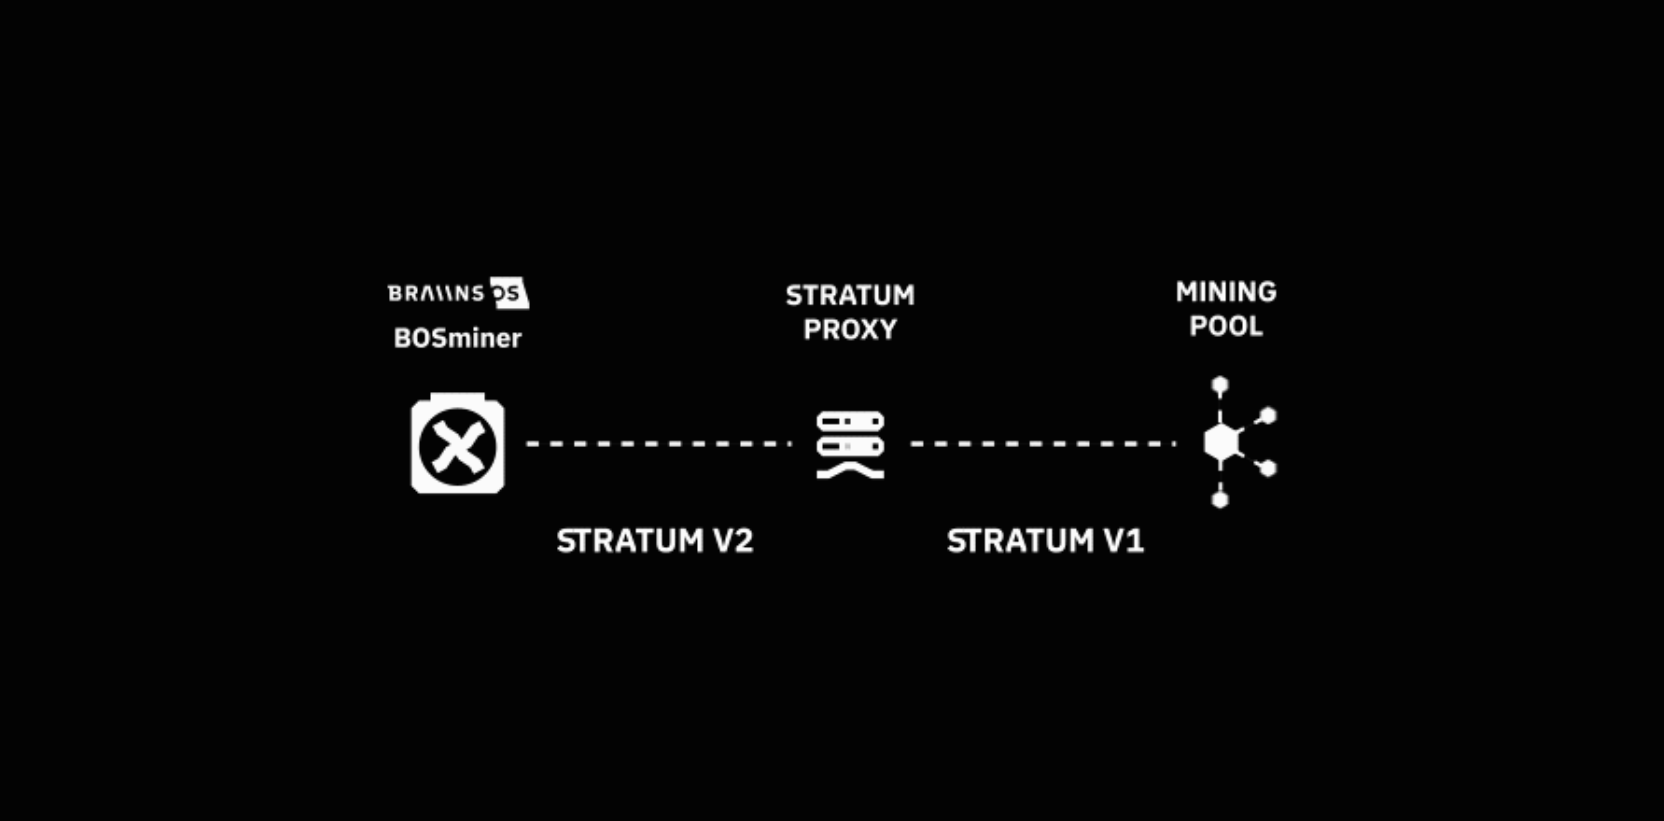
\includegraphics[width=15cm]{Figures/sv2/sv2_7.png}
    \caption{First SV2 implementation released by Braiins team, in 2020}
    \label{fig:sv2_7}
\end{figure}
\noindent Initially, the Braiins team focused on implementing the ASIC protocol logic in the ASIC's firmware, suggesting to use a translation proxy which was in charge of translating the SV2 messages received from the SV2 firmware-miner. As described in \ref{fig:sv2_7}, in that manner the proxy would let the miner communicate correctly with any mining pool which was supporting only Stratum (V1).\\
In that way, any miner could take advantage of the security and data efficiency brought by Stratum V2 protocol, using an encrypted communication channel and the binary framing defined in the SV2 specs.\\

\noindent However, after some months, the Braiins co-founders (co-authors of the SV2 specifications) decided to pass the future development of the protocol to someone who was external to their business. Doing this, they declared that the Stratum V2 protocol implementation should have been done by an independent community, without having the responsibility to be linked in some way to the Braiins company itself.

\subsubsection{\textbf{Stratum Reference Implementation (SRI)}}\label{SRI_intro}
For the above-mentioned reason, during 2020 a new group of people composed by independent developers started to work on a fully open-source implementation of Stratum V2, called SRI (Stratum Reference Implementation).\\
The purpose of SRI group is to build, beginning from the SV2 specifications discussed in the previous section, a community-based implementation, with the aim to discuss and open the development with as many people of the Bitcoin community as possible.

\begin{figure}[h!]
    \centering
    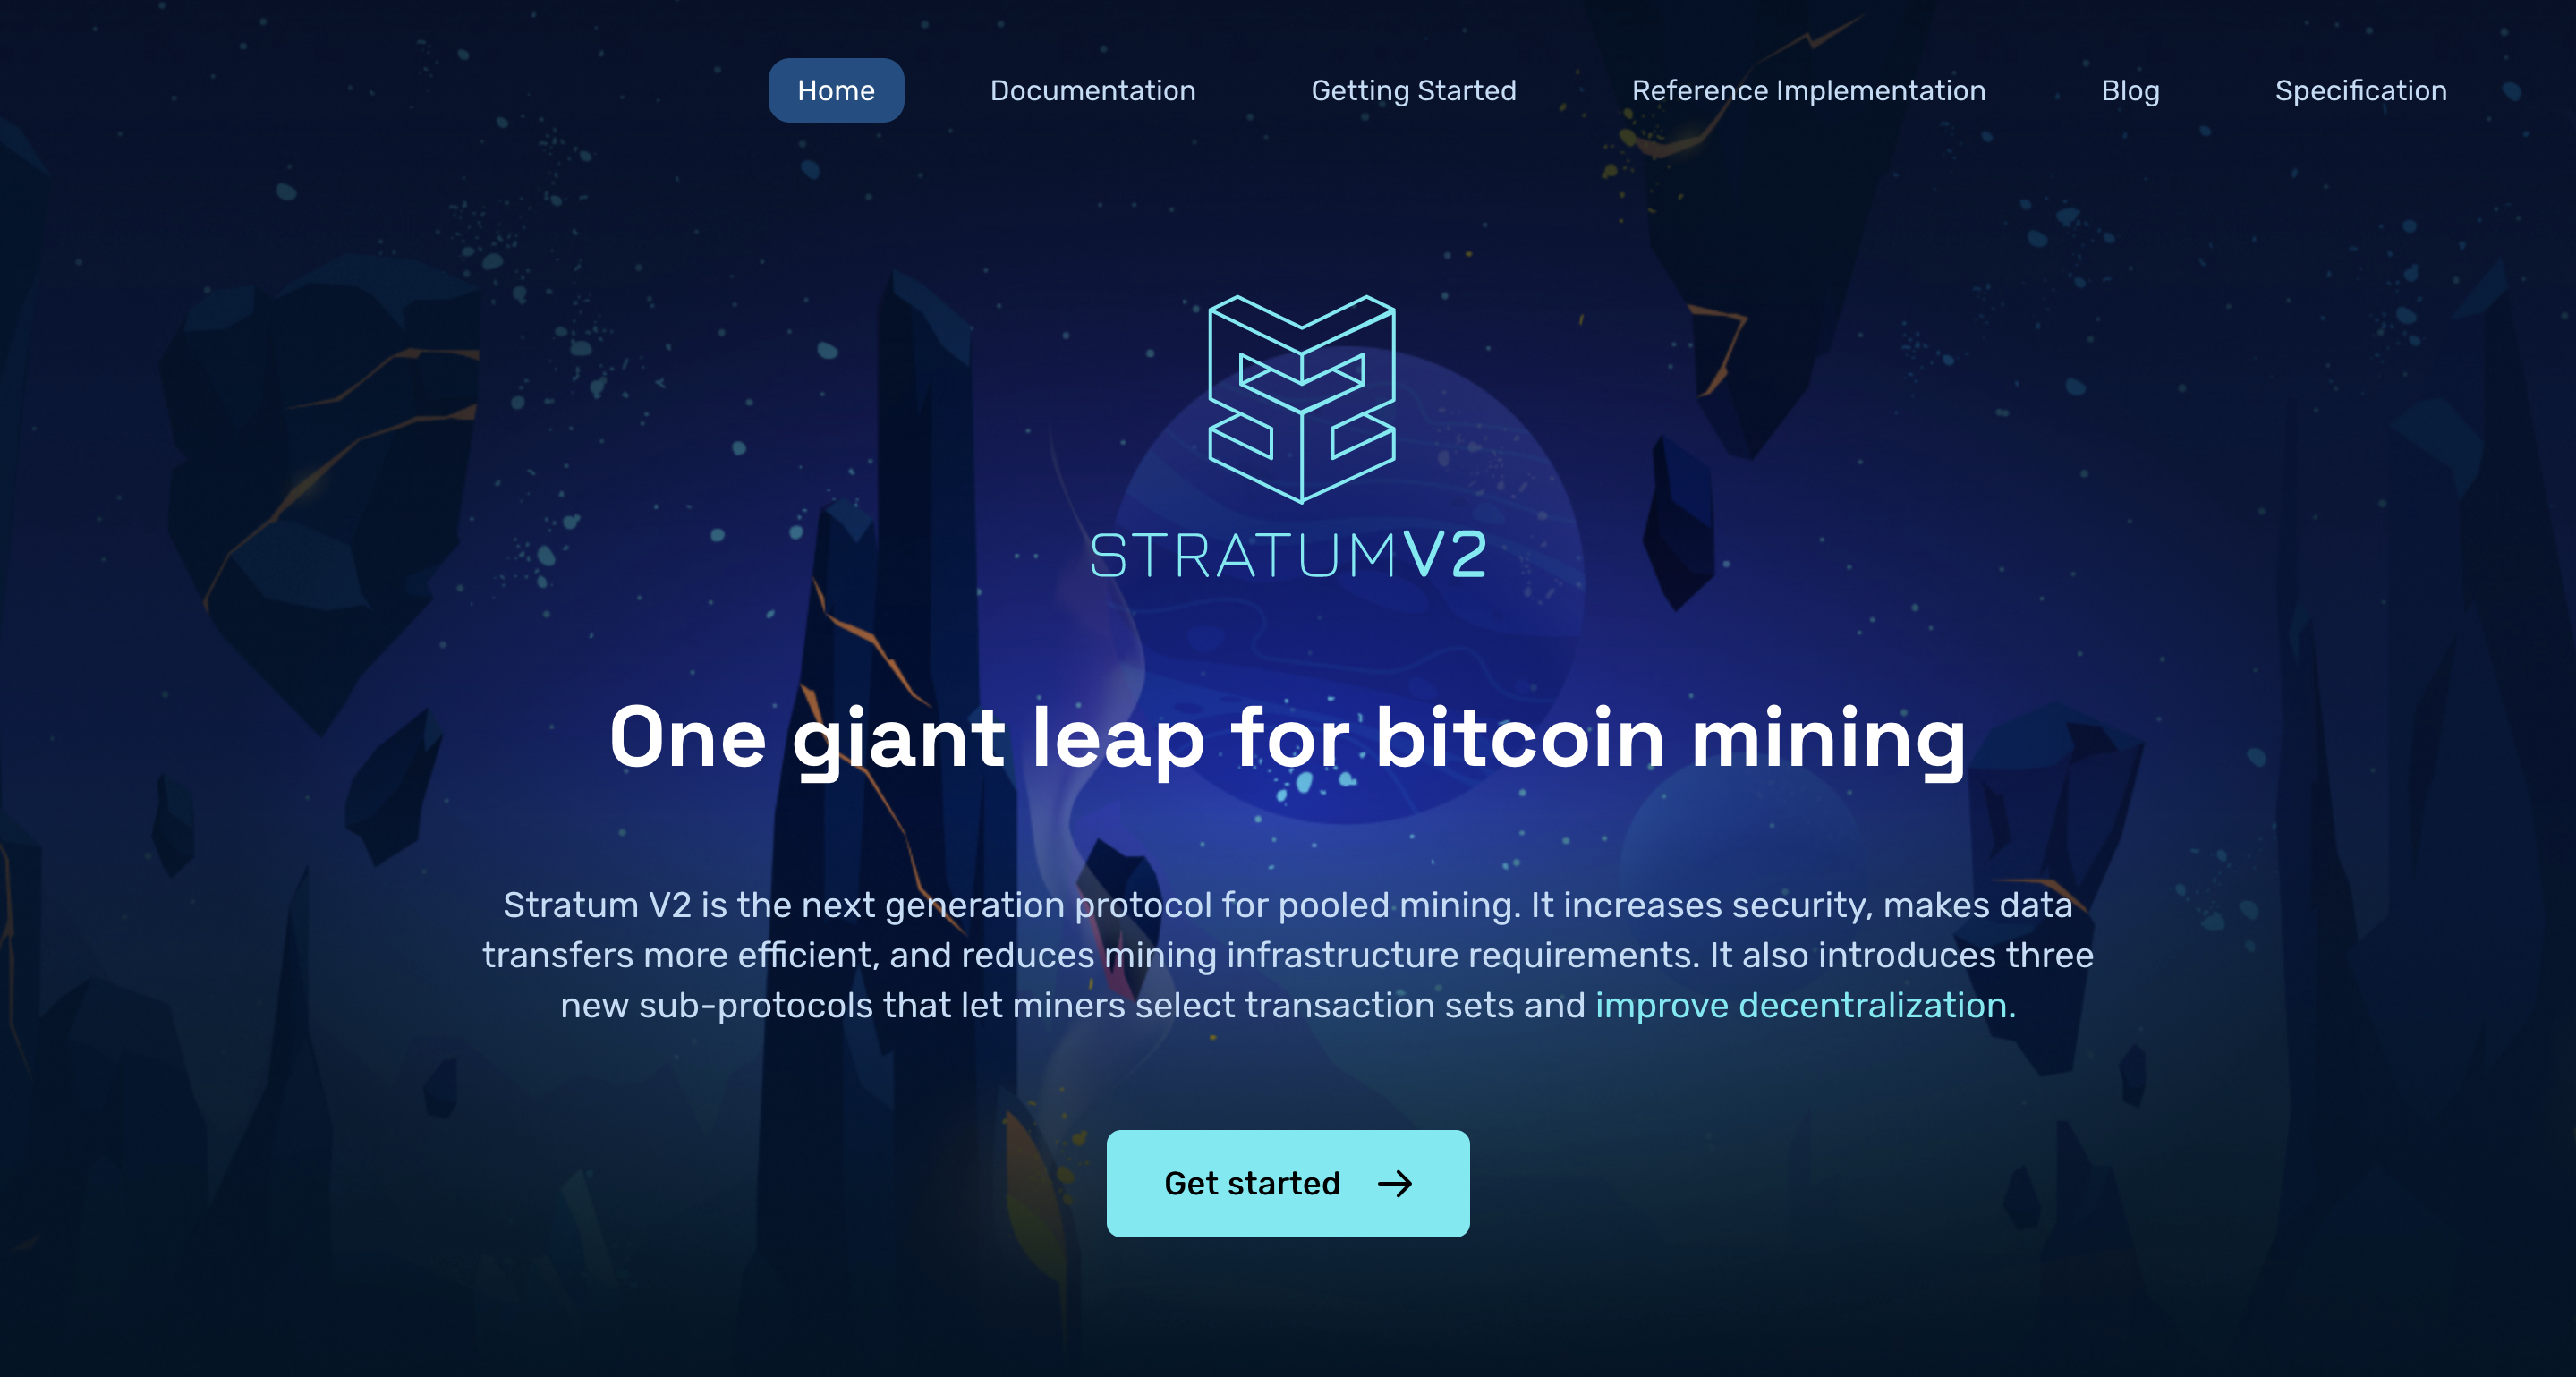
\includegraphics[width=15cm]{Figures/sv2/sv2_8.png}
    \caption{SRI homepage on {\textit{stratumprotocol.org}}}
    \label{fig:sv2_8}
\end{figure}
\noindent In the last year, SRI group did a great work in expanding the SV2 features already covered by the Braiins implementation. \\
For example, they shipped the translator proxy, capable of translating SV1 messages coming from a "SV1" miner to the SV2 logic. Some months ago, SRI group developed and announced the so called \textbf{job-negotiator}, which permits the transaction selection by miners, further decentralizing the power which is currently in the hands of the mining pools operators: <<the new update is "a major milestone in democratizing transaction selections in pooled mining and decentralizing bitcoin," as it allows miners to select transactions via a new sub-protocol and their node.>> \cite{bitcoinmagazinesv2}\\

\noindent In this chapter have been discussed all the major differences between Stratum (V1) and Stratum V2, the enhancements brought by the latter, the new sub-protocols and roles, and the current SV2 implementations.\\\\
In the next chapter, the focus will be about the most important adoption path, which is the Stratum Reference Implementation (SRI). There will be a very deep analysis of the four different configuration which it permits, with a practical part in which two of them will be tested on both cpuminers and real ASIC machines.